\documentclass{article}

\usepackage{graphicx}
\usepackage{tikz}
\usepackage{tikzsymbols}
\usetikzlibrary{calc,patterns,shapes.geometric}
\pagestyle{empty}
\usepackage[margin=0pt]{geometry}
\geometry{papersize={14in,12in}}

\def\centerarc[#1](#2)(#3:#4:#5){\draw[#1] ($(#2)+({#5*cos(#3)},{#5*sin(#3)})$) arc (#3:#4:#5);}

\begin{document}
	\begin{figure}
		\centering
		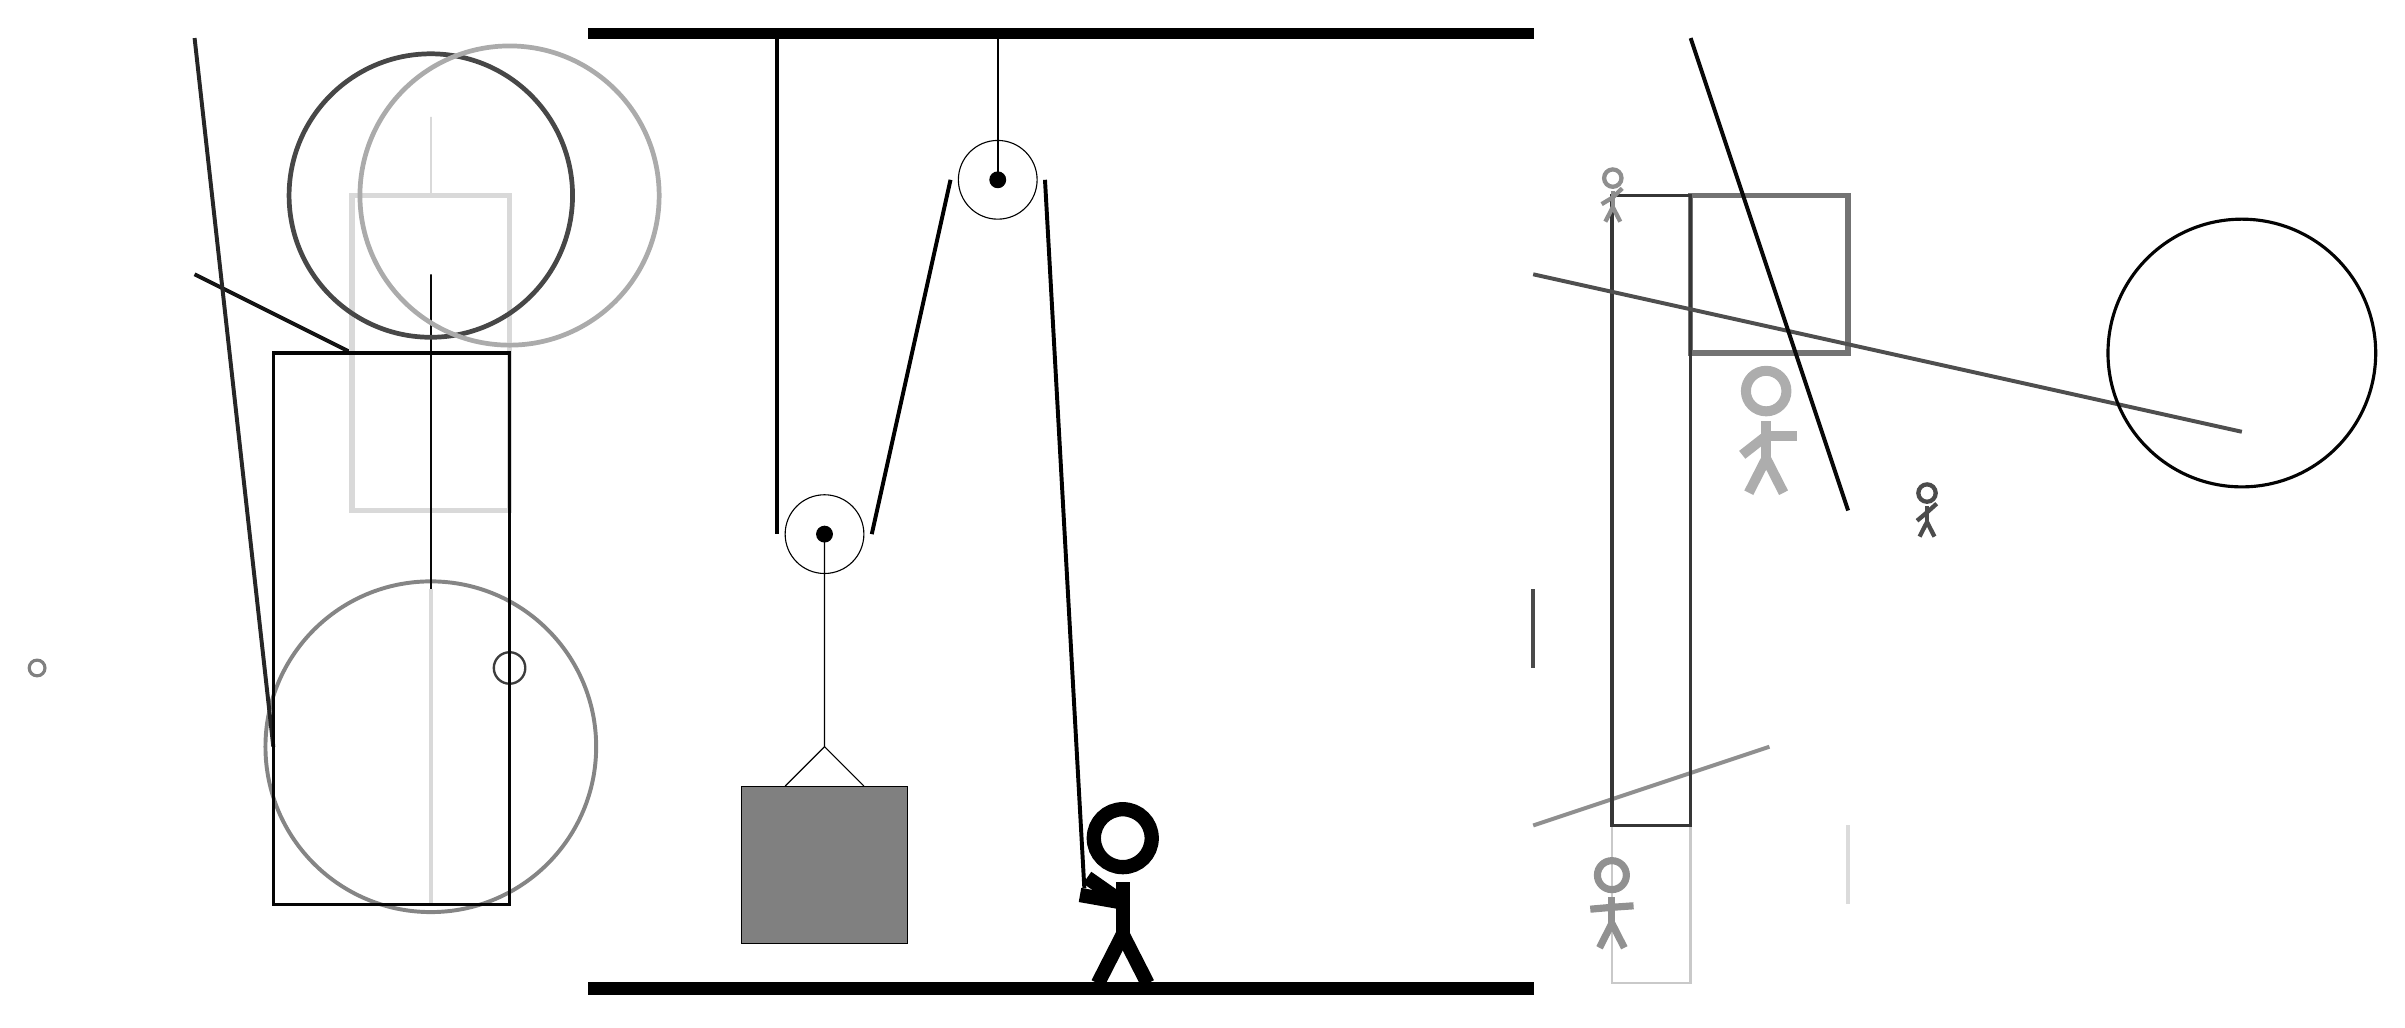
\begin{tikzpicture}
			%%%%% START %%%%%
			
			\draw[fill=black] (-2, 9) rectangle (10, 9.125);
			
			\draw (3.2, 7.2) circle (0.5);
			\draw[fill=black] (3.2, 7.2) circle (0.1);
			\draw[thick] (3.2, 7.2) -- (3.2, 9);
			
			\draw (1, 2.7) circle (0.5);
			\draw[fill=black] (1, 2.7) circle (0.1);
			
			\draw [line width=0.4mm, color=black!50](-9, 1) circle (0.1);
			
			\draw [line width=0.3mm, color=black!76](-3, 1) circle (0.2);
			\draw[line width=0.5mm, color=black!44](13, 0) -- (10, -1);
			\draw[line width=0.3mm, color=black!15] (-4, 7) rectangle (-4, 8);
			\draw[line width=0.5mm, color=black!92](-5, 5) -- (-7, 6);
			
			\draw [line width=0.2mm, color=black!41](12, 8) circle (0.0);
			\draw[line width=0.5mm, color=black!40](-4, 0) -- (-4, -2);
			
			\draw[line width=0.5mm, color=black!71](10, 1) -- (10, 2);
			\draw [line width=0.5mm, color=black!48](-4, 0) circle (2.1);
			\node[line width=0.3mm, color=black!70] at (15, 3) {\Strichmaxerl[3][40][42]};
			\draw[line width=0.3mm, color=black!21] (11, -3) rectangle (12, -1);
			
			\node[line width=0.5mm, color=black!43] at (11, -2) {\Strichmaxerl[5][5][4]};
			\node[line width=0.6mm, color=black!32] at (13, 4) {\Strichmaxerl[7][38][0]};
			\draw[line width=0.5mm, color=black!14](14, -1) -- (14, -2);
			\draw[line width=0.7mm, color=black!15] (-3, 7) rectangle (-5, 3);
			\draw[line width=0.2mm, color=black!97] (-4, 6) rectangle (-4, -2);
			\draw[line width=0.7mm, color=black!55] (12, 7) rectangle (14, 5);
			\draw[line width=0.4mm, color=black!79] (11, 7) rectangle (12, -1);
			\draw[line width=0.5mm, color=black!69](10, 6) -- (19, 4);
			\draw [line width=0.6mm, color=black!72](-4, 7) circle (1.8);
			\draw [line width=0.6mm, color=black!33](-3, 7) circle (1.9);
			
			\node[line width=0.2mm, color=black!44] at (11, 7) {\Strichmaxerl[3][31][44]};
			
			\draw[line width=0.5mm, color=black!85](-6, 0) -- (-7, 9);
			\draw[line width=0.5mm, color=black!15] (-4, 2) rectangle (-4, -2);
			\draw[line width=0.5mm, color=black!97](12, 9) -- (14, 3);
			
			\draw[line width=0.4mm, color=black!98] (-3, -2) rectangle (-6, 5);
			\draw [line width=0.4mm, color=black!99](19, 5) circle (1.7);
			
			\draw (1, 2.7) -- (1, 0) -- (0.5, -0.5);
			\draw (1, 0) -- (1.5, -0.5);
			\draw[fill=black!50] (-0.05, -0.5) rectangle (2.05, -2.5);
			
			\draw[line width=0.5mm] (0.4, 9) -- (0.4, 2.7);
			\centerarc[line width=0.5mm](1, 2.7)(180:360:0.6);
			\draw[line width=0.5mm](1.6, 2.7) -- (2.6, 7.2);
			\centerarc[line width=0.5mm](3.2, 7.2)(0:180:0.6);
			\draw[line width=0.5mm](3.8, 7.2) -- (4.3, -1.8);
			
			\node at (4.7, -1.9) {\Strichmaxerl[10][-35][170]};
			
			\draw[fill=black] (-2, -3) rectangle (10, -3.15);
			
			%%%%% END %%%%%
		\end{tikzpicture}
	\end{figure}	
\end{document}